\documentclass[twocolumn]{article}
\usepackage{graphicx}
\usepackage{amsmath}
\usepackage{float}
\usepackage{amssymb} %Use of therefore symbol
\usepackage{hyperref}
\usepackage{caption}



\begin{document}
\title{Lab / Assignment 3: Differential Equations}
\author{Alex Matheson, Austin Nhung}
%\affiliation{Department of Physics and Astronomy, University of Calgary, Calgary AB T2N 1N4 Canada}
\date{\today}
\maketitle

\section{Introduction}
Differential equations form the backbone of most physics sub-disciplines. Substantial work has been put into analytically evaluating these equations. With the exception of some symbolic languages, computers cannot employ the continuity that analysis requires; methods must be used that convert continuous differential equations to some discrete form. Finite differences uses the formal definition of the derivative to create different equations called 'stencils' that relate a value at a point to values at other discrete points. This lab explored many different stencils that were devised to minimise error, overcome discrete limitations, and counteract phenomena that may artificially arise as a side effect of discretisation. 

\section{Methods}
\subsection{Warm-Up}
Finite differences allows one to set up an equation relating the value of a variable at a point to the values in the surrounding discrete locations. For instance, a two dimensional Laplace equation of the form $u_{xx} + u_{yy} = 0$ would have the form $u_{i+1,j} + u_{i-1,j} + u_{i,j+1} + u_{i,j-1} - 4u_{i,j} = 0$. By re-writing this equation in terms of $u_{i,j}$, we can have a series of equations that define the value of each point relative to that of its neighbors. If boundary values are supplied, this yields $n\times m$ equations for a region divided into $n+2$ x-points and $m+2$ y-points. The \textbf{direct method} is used to solve this system of equations exactly, by solving the series of equations using matrix methods such as Gaussian methods or L-U decomposition. Direct methods however may not always be desirable. This is because the matrix solving algorithms used may be slow and inefficient. Additionally, some data sets may not behave well with certain matrix methods computationally. As a result of this, iterative methods have been developed to address these shortcomings.

Iterative methods involve "guessing" a solution to the equation, and then continually refining the results until they converge to a solution (note that convergence tests may be required to ensure that the system converges to the correct solution). Given a series of boundary values, the inner values may then all be guessed. Next, finite differences may be used to determine an equation that defines the value of a cell based on its neighbors. Whereas the direct method tried to simultaneously determine all cells, the iterative starts with a guess, then uses the  finite difference equation to create a new "generation" of grid based on the previous grid's values. In the earlier example, this equation would be $u_{i,j}^{k+1} = (u_{i+1,j}^{k} + u_{i-1,j}^{k} + u_{i,j+1}^{k} + u_{i,j-1}^{k})/4 $ where $k$ signifies the current iteration of the system. This method continues until certain criteria are met, though the final result will have some associated error. The method benefits, however, by generally performing faster than direct methods, especially when the guess is close to the actual answer.

There are different ways to implement iterative methods. The Jacobi method is closest to what has been described so far. In the Jacobi method, the grid is solved at some iteration $k$. Once the iteration is complete, the system is compared to exit conditions, and then the next iteration is generated. The Gauss-Seidel method considers a different approach. We know that the more iterations take place, the more likely a value at a particular point is to be correct. For the first point in a grid we consider, we use all the neighbor values from the previous iteration. In the Jacobi method, the next point also uses all the neighbor points from the previous iteration. The Gauss-Seidel method realizes that for the second point, we already have one "updated" point that should be closer than the previous iteration, so we use the updated neighbor when available instead of the previous iteration to approach the solution more quickly. In practice, the Gauss-Seigel method uses a checkerboard scheme, where points alternate between usng only previous iteration values and using a mixture of previous -  and current iteration values. This scheme maximizes the number of updated points used in the calculation, speeding up the algorithm. The Jacobi method is more intuitive to implement, since it completes one iteration at a time. The Jacobi method can also be split apart into different intersecting independent grids for parallelization, whereas the Gauss-Seigel method cannot be parallelized easily.

The aforementioned methods can be used to solve numerous physical systems. Many differential equaitons have general forms that have been given names over time.

\begin{table*}
\begin{center}
\begin{tabular}{|c|c|c|}
	\hline Name                        & Form                                & Order \\ 
	\hline Poisson's equation          & $\nabla^2 u = f(x,y,z)$             & 2 \\ 
	\hline Laplace's equation          & $\nabla^2 u = 0$                    & 2 \\ 
	\hline 3-Dimensional Wave equation & $u_{tt} = c^2\nabla^2 u$            & 2 \\ 
	\hline 1-Dimensional Heat equation & $u_t -\alpha u_{xx} = 0$            & 2 \\ 
	\hline 1-Dimensional Wave equation & $u_{tt} = c^2 u_{xx} $              & 2 \\ 
	\hline Ginzburg-Landau equation    & $A_t = A_{xx} + \sigma A - |A|^2 A $& 2 \\ 
	\hline Korteweg-de Vries equation  & $u_t + u_{xxx} - 6u u_{x} = 0 $     & 3 \\ 
	\hline 
\end{tabular}  
\caption{Different types of differential equations, their general forms, and order.}
\label{eq:diff_equations}
\end{center}
\end{table*}

Differential equations may be classified according to the descriminant of the generalized form $au_{xx} + bu_{xy} + cu_{yy} + du_{x} +eu_y +fu + g =0$. A zero discriminant is classified as parabolic, whereas positive and negative are hyperbolic and elliptic respectively. Based on this, three sample PDEs may be considered. The equation $u_{tt} = 2u_{xx}$ is hyperbolic with a discriminant of 8, $u_{xx} + u_{yy} = 0$ is elliptic with a discriminat of -4, and $u_t - u_{xx}$ is parabolic with a discriminant of 0.

There are three different first order FD operators that may be used on a function. For the function $u(x)=x^2$, the forward FD is as follows:
\begin{equation}
\begin{split}
\partial_x^+ u =& \frac{u(x+h) - u(x)}{h} \\
\partial_x^+ u(3) =& \frac{u(3+0.1) - u(3)}{0.1} \\
\partial_x^+ u(3) =& \frac{9.61-9}{0.1} \\
\partial_x^+ u(3) =& 6.10 \\
\end{split}
\end{equation}
With a finer grid resolution, the result becomes:
\begin{equation}
\begin{split}
\partial_x^+ u =& \frac{u(x+h) - u(x)}{h} \\
\partial_x^+ u(3) =& \frac{u(3+0.05) - u(3)}{0.05} \\
\partial_x^+ u(3) =& \frac{9.3025-9}{0.05} \\
\partial_x^+ u(3) =& 6.0500 \\
\end{split}
\end{equation}
In both cases, the result is near the expected result of 6, but is off by a single factor of $h$. This matches the error of order $O(h)$ for the forward method. 

Another FD method is the central method. The same two examples may be computed using this method.
\begin{equation}
\begin{split}
\partial_x u =& \frac{u(x+h) - u(x-h)}{2h} \\
\partial_x u(3) =& \frac{u(3+0.1) - u(3-0.1)}{2*0.1} \\
\partial_x u(3) =& \frac{9.61-8.41}{0.2} \\
\partial_x u(3) =& 6.00 \\
\\ 
\partial_x u =& \frac{u(x+h) - u(x-h)}{2h} \\
\partial_x u(3) =& \frac{u(3+0.05) - u(3-0.05)}{2*0.05} \\
\partial_x u(3) =& \frac{9.3025-8.7025}{0.1} \\
\partial_x u(3) =& 6.000 \\
\end{split}
\end{equation}
As expected according to the text, the central method was more accurate. The result matched the analytical solution exactly.

%SHOW IT IS SECOND ORDER ACCURATE
\begin{thebibliography}{00}
	\bibitem{ouyed}
	Ouyed and Dobler, PHYS 581 course notes, Department of Physics and Astrophysics, University of Calgary (2016).
	\bibitem{NR}
	W. Press et al., \emph{Numerical Recipes} (Cambridge University Press, 2010) 2nd. Ed.
	\bibitem{pulsar}
	T. O'Brian, "Properties of Pulsars", University of Manchester Jordell Bank Observatory, accessed at \url{http://www.jb.man.ac.uk/distance/frontiers/pulsars/section1.html}.
	\bibitem{sunspots}
	D. Hathaway, "The Sunspot Cycle",  NASA, accessed at \url{ https://solarscience.msfc.nasa.gov/SunspotCycle.shtml}
\end{thebibliography}

There are many different finite difference schemes that may be employed. Table \ref{schemes} shows many of the different schemes covered in the course. 

\begin{table*}
	\begin{center}
		\begin{tabular}{|c|c|c|c|}
			\hline
			Name & FD Scheme & Order & CFL \\
			\hline
			Forward Euler & $u_{k}^{l+1} = u_k^l +r(u_{k+1}^l - u_k^l) $ & 1 & $r\leq 1$ \\
			\hline
			Upwind & $ u_{k}^{l+1} = u_k^l -|r|(u_k^l - u_{k-1}^l) $ & 1 & $r\leq 1$ \\
			\hline
			Leap Frog & $u_{k}^{l+1} = u_k^{l-1} +r(u_{k+1}^l - u_{-1}^l) $ & 2 & $r\leq 1$ \\
			\hline
			Lax-Wendoff & $u_{k}^{l+1} = u_k^l - \frac{r}{2}(u_{k+1}^l - u_{k-1}^l) + \frac{r^2}{2}(u_{k+1}^l - 2u_k^l + u_{k-1}^l) $ & 2 & $r\leq 1$ \\
			\hline
			Backward Euler & $u_{k}^{l+1} = (1 + r)^{-1}(u_k^l + ru_{k+1}{l+1}) $ & 1 &  None\\
			\hline
			Crank-Nicholson & $u_{k}^{l+1} = u_k^l +\frac{r}{2 \Delta x}(u_{k+1}^{l+1} - 2u_k^{l+1} +u_{k-1}^{l+1} + u_{k+1}^l -2u_k^l + u_{k-1}^l) $ & 2 & None \\
			\hline
		\end{tabular}
		\label{Schemes}
		\caption{Different FD schemes, their respective orders and stabilities. The variable $r$ has been used to represent the Courant number $c\Delta t / \Delta x$. The Last two schemes are implicit, while the rest are explicit.}
	\end{center}
\end{table*}

Of the schemes covered, they could be divided into two types: explicit and implicit. Explicit schemes may be solved cell-by-cell. That is, a cell at time $l+1$ could be found using a single equation, since it was dependant only on cells at time $l$. Implicit schemes on the other hand, require that the values in all cells be solved simultaneously, since a variable at time $l+1$ will be dependant on the values in other cells at time $l+1$ in such schemes. Implicit schemes therefore require the use of linear algebra to solve equations simultandously, usually using some matrix-solving method such as LU decomposition. Implicit schemes have the benefit of always being stable, meaning one is free to chose time and space resolutions as one wishes. The downside of the implicit method is that simultaneous solving is more computationally expensive. One needs to weigh the tradeoff between run-time and resolutions when deciding on a method to use. 

In the previous paragraph, stability of a discrete approximation was touched upon. A simulation becomes unstable if its values begin to explode contrary to physical conservation laws. Given enough time, the values of the variable of interest will explode to infinity. This instability is the result of selecting certain grid spacings that prevent proper transfer of information. To determine when a scheme becomes unstable, Von Neumann stability analysis may be applied. Von Neumann stability analysis takes advantage of the Fourier representation of a function. Out value $u$ is some linear sum of waves. At some future time $u^{l+1}$ our system should be the same set of waves, but evolved. This may be represented as a constituent wave being multiplied by some factor $A$. If $A>1$, then after some period of time, that constituent wave will dominate the variable, and explode to infinity. The Van Neumann method therefore determines the domain of such amplitudes, and determines under what conditions $A>1$. By plugging in the Fourier representation of a variable into our finite difference stencil, we may re-arrange to determine the value of A with respect to the courant number.

% DERIVE A VAN NEUMANN STABILITY HERE

\subsection{Time Independent PDEs}
\subsubsection{Relaxation Methods}

The laplacian equation was considered as an example of a time independent PDE. The equation could be converted into a stencil as shown below:
\begin{equation}
\begin{split}
u_{xx} + u_{yy} &= 0 \\
\frac{u_{i+1,j} - 2u_{i,j} + u_{i-1,j}}{(\Delta x)^2} + \frac{u_{i,j+1} - 2u_{i,j} + u_{i,j-1}}{(\Delta{y})^2} =&0 
\end{split}
\end{equation}
If the grid spacing in each dimension is equal, the denominators may vanish yielding:
\begin{equation}
u_{i+1,j} + u_{i-1,j} + u_{i,j+1} + u_{i,j-1} - 4u_{i,j}=0
\end{equation}
These equations may be solved using matrix methods, given some boundary conditions, or may be solved iteratively. Iterative solving uses the notion that the limit of $\partial u/ \partial t$ should be zero for a time independent system. Therefore, setting non-boundary values to some initial guess should yield a correct solution if the zero in the Laplace stencil is replaced with  $\partial u/ \partial t$ and allowed to evolve for sufficient time. 

The iterative method was tested using a set of boundary conditions $u(x,0) = u(x,10.0) = u(0.0,y)=0$ and $u(20.0,y)=100.0$. The system was tested beginning with a resolution $\Delta x = \Delta y = 5.0$. A code was written to evaluate and display this. Figure \ref{fig:low_res_iterative} shows the results of this system. The result was extremely low resolution, and was thus liable to be innacurate compared to the analytical solution. To improve the accuracy, the resolution of the system was successively doubled four times. This is shown in figure \ref{fig:relaxation}. 

\begin{figure}
\centering
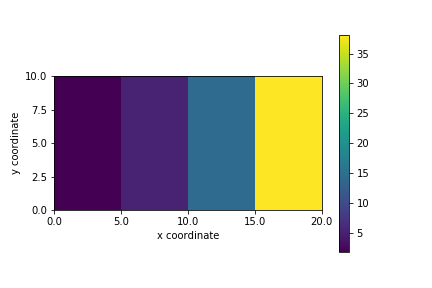
\includegraphics[width=\linewidth]{low_res_iterative}
\caption{Solution to the Laplace equation for a set of boundary conditions. The wall at $x=20.0$ is set to $u=100.0$ while the other edges are set to $u=0$. The image is low-resolution, measuring $2\times4$ cells.}
\label{fig:low_res_iterative}
\end{figure}

\begin{figure}
\centering
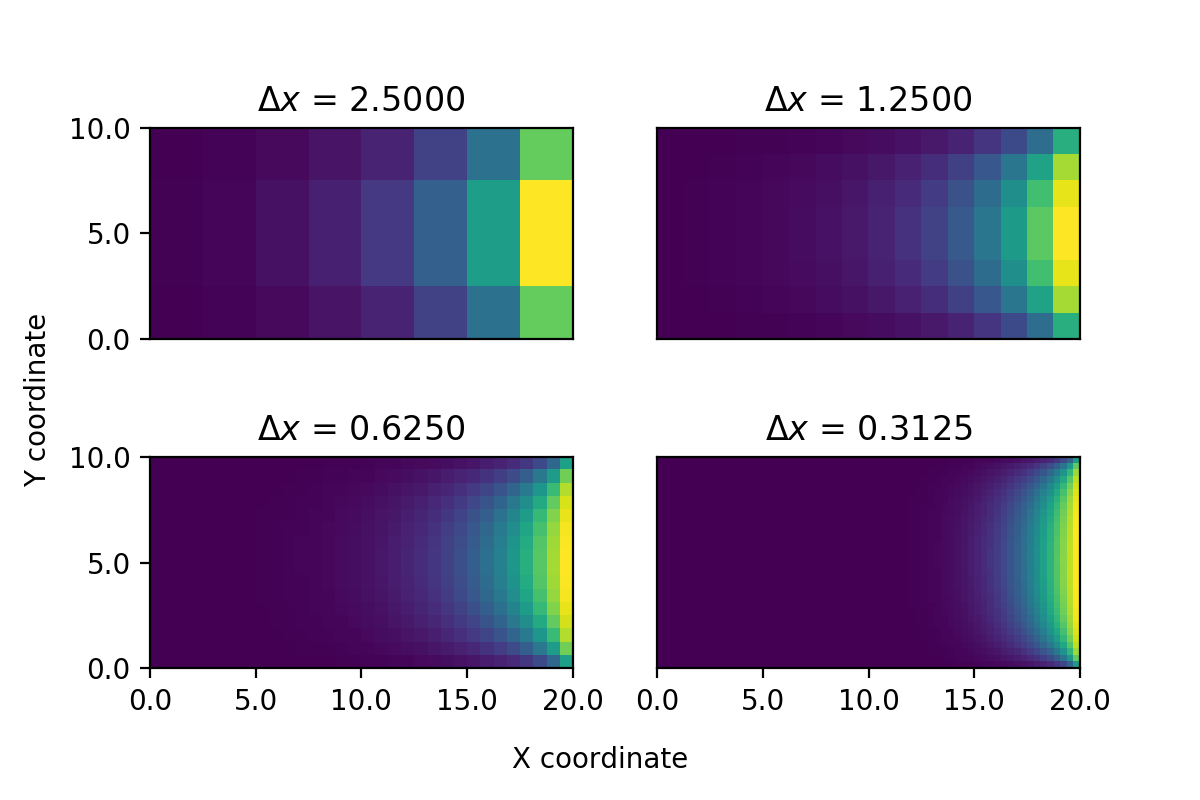
\includegraphics[width=\linewidth]{relaxation}
\caption{Solution to the same Laplace system as figure \ref{fig:low_res_iterative}. The system has been evaluated at a higher resolution for each successive panel.}
\label{fig:relaxation}
\end{figure}

The Laplacian equation is present in many physical systems. An example of the voltage inside a capacitor was considered. Boundary conditions along the plates were considered:
\begin{equation}
\begin{split}
u(x,0) &= 100\sin(\frac{2\pi x}{L}) \\
u(x,1) &= -100\sin(\frac{2\pi x}{L}) \\
u(0,y) &= u(L,y) - 0
\end{split}
\end{equation}
Where the plates were of width $L$ and placed a distance of $L$ apart. The problem was approached using two variations of the relaxation method. The first was the Jacobi method, which was used in the previous problem. The second was the Gauss-Seidel method. The Gauss-Seidel method should be more efficient, as it uses an updated cell value during its sweeps if there is an updated value for one of the stencil cells. The results of the two methods are shown in figure \ref{fig:capacitor_methods}. To test which method converged to a solution faster, a convergence criterion was used. Once no cell on the grid was more than $10^{-8}$ in difference from the previous iteration, the result was considered correct. The Jacobi method converged after $5390$ iterations, while the Gauss-Seidel method converged after $3809$ iterations.

\begin{figure}
\centering
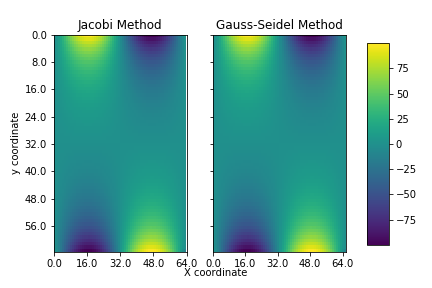
\includegraphics[width=\linewidth]{capacitor_methods}
\caption{Final solutions obtained for a capacitor voltage problem using the Jacobi and Gauss-Seidel methods. Both methods yielded the same result. Note that axes are not to scale.}
\label{fig:capacitor_methods}
\end{figure}

\subsubsection{The Schr\"{o}dinger Equation}
This section considered a common model for the Schr\"{o}dinger equation that was a variant of the Laplace equation:
\begin{equation}
\frac{\partial^2 u}{\partial x^2} + \frac{\partial^2 u}{\partial x^2} - \alpha u = 0
\end{equation}

The stencil for this differential equation was largely similar to that of the Laplace equation, with a single added term. The stencil is as follows:
\begin{equation}
	u_{i+1,j} + u_{i-1,j} + u_{i,j+1} + u_{i,j-1} - 4u_{i,j} -\alpha u_{i,j}=0
\end{equation}

As previously mentioned, this system may be solved as a series of linear equations using matrix methods. To demonstrate this solution, the problem was considered for a square of length $1$, resolution $50\times50$, with $u$ at all boundaries set to $1$. A python script was written to evaluate the system of equations, by flattening the 2D $u$ array into a one dimensional array. Next, the stencil was also flattened into a $50^2 \times 50^2$ 2D matrix. These terms could then be used to solve an $A\mathbf{x} = \mathbf{b}$ system. The script was made more quickly using a variant of LU decomposition for banded matrices that sped the execution time to approximately $1.3$ seconds. The result is shown in panel 1 of figure \ref{fig:schroe_alpha_1}.

Another method used to evaluate such systems was a weighted Jacobi method. In essence, the method weights how heavily to consider the stencil terms rising from the time derivative versus how heavily to consider the stencil terms from the spacial derivatives. A series of 5 weighting coefficients were examined for the same problem as above with $\alpha = 1$. The results of this method are shown alongside the direct method in figure $\ref{fig:schroe_alpha_1}$. The method was also tested for a variant equation with $\alpha=1000$. The com

\begin{table*}
	\begin{center}
\begin{tabular}{|c|p{2cm}|p{2cm}|p{2cm}|p{2cm}|}
	\hline  Method& Time to compute $\alpha=1$ & Iterations to compute $\alpha=1$ & Time to compute $\alpha=1000$ & Iterations to compute $\alpha = 1000$ \\ 
	\hline
	Direct & 0.28s & 1  & 0.24s & 1 \\ 
	\hline
	Weighted $w=0.1$  & 327.8s & 30000 & 11.8s & 1039 \\ 
	\hline
	Weighted $w=0.25$  & 264.8s  & 22529 & 4.81s & 446\\ 
	\hline
	Weighted $w=0.5$  & 144.9s & 11956 & 2.46s & 232 \\ 
	\hline
	Weighted $w=0.75$  & 95.1s & 8239 & 1.68s & 158 \\ 
	\hline
	Weighted $w=0.9$  & 75.9s & 6967 & 1.44s & 132\\ 
	\hline 
\end{tabular} 
\caption{Computation Speed of both the direct and weighted Jacobi methods. The weighted Jacobi method would had an iteration exit condition of $30000$ loops.}
\label{Jacobi compare}
	\end{center}
\end{table*}

\begin{figure*}
\centering
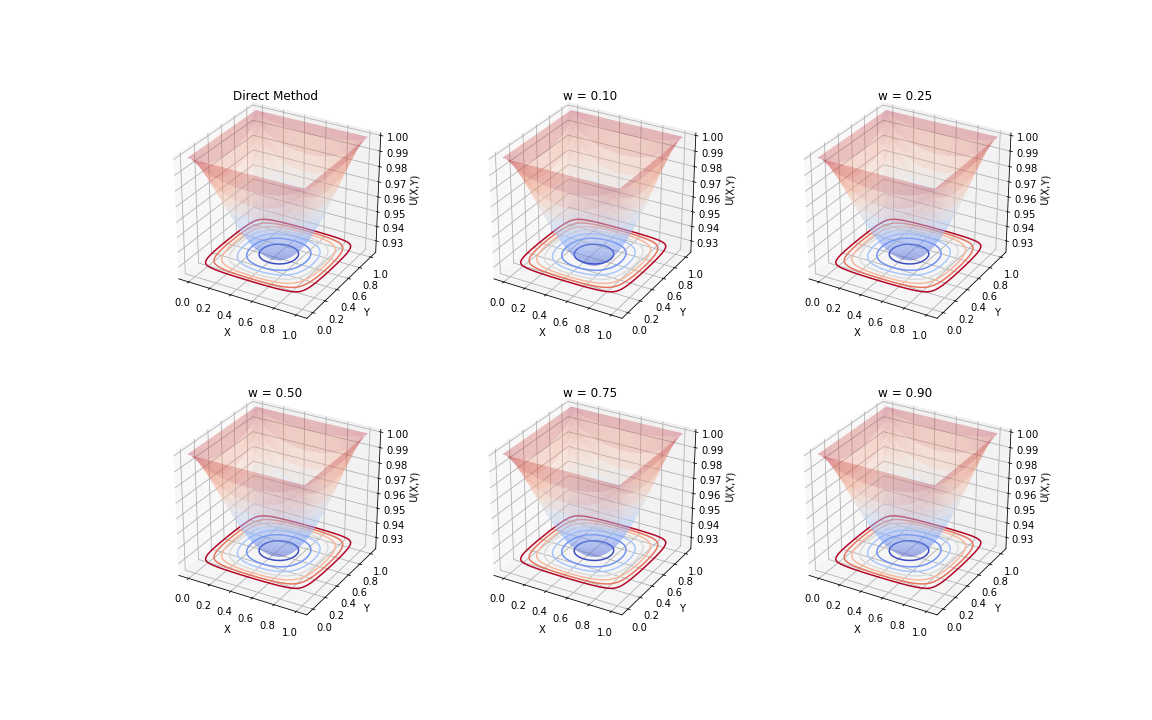
\includegraphics[width=\textwidth]{schroe_alpha_1}
\caption{Solution to a model Schr\"{o}dinger equation with $\alpha=1$. All methods produced aproximately the same result, with the only difference being in computation time.}
\label{fig:schroe_alpha_1}
\end{figure*}

\begin{figure*}
	\centering
	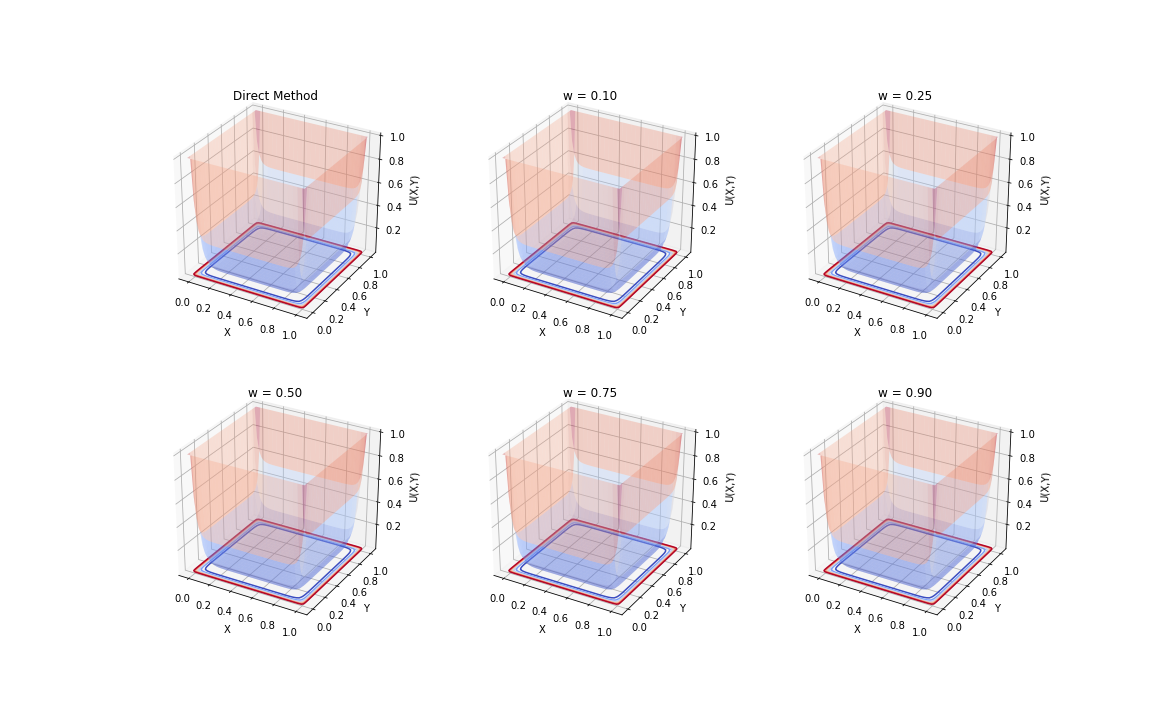
\includegraphics[width=\textwidth]{schroe_alpha_1000}
	\caption{Solution to a model Schr\"{o}dinger equation with $\alpha=1000$. All methods produced aproximately the same result, with the only difference being in computation time.}
	\label{fig:schroe_alpha_1000}
\end{figure*}

\subsection{Hydrodynamics}
\subsubsection{Code Introduction}

An example of rigorous code that simulates hydrodynamics in 2 dimensions was provided for the purposes of this lab. The code simulates the pressure, flow velocity, and density of a fluid or gas using the Navier-Stokes equations and related advection, diffusion, and dispersion terms such as those described in this lab. The code takes advantage of a staggered mesh. A staggered mesh is where different quantities are not evaluated at the same points, and instead are stored in separate meshes. In the case of this code, the scalar quantities (density, pressure) were located co-locally and the vector quentities (x and y flow velocity) were located at half steps to either side of the scalars. This functioned as the scalars being located in the middle of some unit cell, and the vectors (used as a flux quantity) located at the faces of the unit cube. Staggered grids are desirable, as they eliminate odd-even decoupling that can occur in co-local schemes.

As the code provided was written in Fortran, it required compilation. The various dependencies in the source code were managed using a makefile. This makefile was written to compile the code, create a new sub-directory containing set-up documents, and to clean directories of old compiled versions. 

The code provided contained a default implementation of four initial high pressure points that were then allowed to diffuse. The code was compiled and allowed to run. Figure \ref{fig:drops} shows the resulting behaviour. The pressurized points diffuse as expected. When encountering the obstacle, the pressure waves appear to reflect. No reflections occurred at the edges, indicating that matter in the simulation zone was allowed to leave the active zone and flow out.

\begin{figure}
\centering
\includegraphics[width=\linewidth]{phys581-Lab3-package-2018/exe-dir/drops}
\caption{Initial configuration of the hydrodynamics simulation. Initial conditions specify four high pressure zones. No additional forcing was provided, and the subsequent frames allow the pressure zones to disperse. A square obstacle has been placed at the centre of the active zone, and can be seen as a solid zone of colour when pressure disturbances approach.}
\label{fig:drops}
\end{figure}

\subsubsection{CFL Condition}
The code as distributed did not have a proper CFL condition implemented. This prevented the code from running at an optimal speed. In order to compute the CFL at any given step, the speed of sound everywhere must be known. The speed of sound may be defined by the equation:
\begin{equation}
c_s = \sqrt{(\frac{\partial p}{\partial \rho})_s}
\end{equation}
A further equation used by the simulation used an adiabiatic equation to define the pressure relative to the density:
\begin{equation}
p = \rho^\gamma
\end{equation}
These two equations were combined to determine the speed of sound, with the adiabatic index $\gamma = 5/3$:
\begin{equation}
c_s = \sqrt{(\frac{\partial p}{\partial \rho})_s} = \sqrt{\gamma \rho^{\gamma-1}}
\end{equation}
The code manipulates this result to take both pressure and density into account, by re-substituting pressure:
\begin{equation}
\sqrt{\gamma \rho^{\gamma-1}} = \sqrt{\frac{\gamma \rho^\gamma}{\rho}} = \sqrt{\frac{\gamma p}{\rho}}
\end{equation}

To implement this CFL condition, the general 2D CFL condition was used:
\begin{equation}
C = \frac{u_x \Delta t}{Delta x} + \frac{u_y \Delta t}{\Delta y}
\end{equation}
Where $u$ is the speed of the medium in that direction, which will usually be c_s. This could be re-arranged using $C=0.5$ to find $\Delta t$ at each step. Important to note is that $u$ is not the same at all points being simulated. To determine the $u$ value to use, the maximum $u$ occurring in the grid must be used. This maximum value is either the speed of sound, or the highest flow speed in the medium, whichever is higher. 

The CFL file was modified to determine both the maximum speed and the CFL condition using the speed of sound equation defined above. Before running the CFL condition, the default simulation running to $t=10.0$ took $135.7s$ with an improper $dt=10^{-3}$. After implementing dynamic CFL, the same simulation took $14.1s$. The speed difference is due to the CFL condition choosing the highest $dt$ possible without causing instability. This allows the system to reach its time-goal much more quickly in runtime. 

\subsubsection{Injection Inlet}
Once the simulation was optimized, physical situations could be modeled. One such application is a wind-tunnel, where a stream of high velocity fluid is injected from the left. The 

% FIGURES OF JET, COMMENTS ON DIFFERENT DENSITIES

Once the jet was established, different solid shapes could be placed in the path of the jet in order to examine aerodynamic properties. First, built-in subroutines were used to place a vertical wall in the path of the jet. 

\subsubsection{Airplane Aerodynamics}


\section{Discussion}

\section{Conclusion}


\section{Appendix}
For access to the source codes used in this project, please visit \url{https://github.com/Tsintsuntsini/PHYS_581} for a list of files and times of most recent update.
	
\end{document}